\documentclass[
	article,
	11pt,
	oneside,
	a4paper,
	english,
	brazil,
	sumario=tradicional
	]{abntex2}

\usepackage{lmodern}
\usepackage[T1]{fontenc}
\usepackage[utf8]{inputenc}
\usepackage{indentfirst}
\usepackage{nomencl}
\usepackage{color}
\usepackage{graphicx}
\usepackage{microtype}
\usepackage[brazilian,hyperpageref]{backref}
\usepackage[alf]{abntex2cite}
\usepackage[makeroom]{cancel}
\usepackage{amsmath, amssymb}
\usepackage{mathtools}
\usepackage{esint}
\graphicspath{{img/}}

\newcommand{\norm}[1]{\left\lVert#1\right\rVert}
\renewcommand{\backrefpagesname}{Citado na(s) página(s):~}
\renewcommand{\backref}{}
\renewcommand*{\backrefalt}[4]{
	\ifcase #1
		Nenhuma citação no texto.
	\or
		Citado na página #2.
	\else
		Citado #1 vezes nas páginas #2.
	\fi}

\titulo{Projeto 03 - Anel Carregado}
\tituloestrangeiro{}

\autor{Equipe Donner
\\[0.5cm]
Diogo Silva, Guilherme Shimada, Leonardo Vieira, Lucca Miranda, Pedro Azevedo}

\local{Brasil}
\data{17 de Novembro, 2021}

% alterando o aspecto da cor azul
\definecolor{blue}{RGB}{41,5,195}

\makeatletter
\hypersetup{
	pdftitle={\@title},
	pdfauthor={\@author},
	pdfsubject={Modelo de artigo científico com abnTeX2},
	pdfcreator={LaTeX with abnTeX2},
	pdfkeywords={abnt}{latex}{abntex}{abntex2}{atigo científico},
	colorlinks=true,
	linkcolor=blue,
	citecolor=blue,
	filecolor=magenta,
	urlcolor=blue,
	bookmarksdepth=4
}

\makeatother
\makeindex
\setlrmarginsandblock{1.5cm}{1.5cm}{*}
\setulmarginsandblock{1.5cm}{1.5cm}{*}
\checkandfixthelayout

\setlength{\parindent}{1.3cm}
\setlength{\parskip}{0.2cm}
\setlength{\columnsep}{1.0 cm}
\SingleSpacing

\begin{document}

\selectlanguage{brazil}
\frenchspacing

\twocolumn[ % INICIO DE ARTIGO EM DUAS COLUNAS
\maketitle

\begin{resumoumacoluna}

Este artigo apresenta uma discussão teórica a respeito do comportamento de um anel de material isolante carregado e imerso em um campo magnético variável. Para esse propósito, apresentaremos equações que descrevem esse corpo no ambiente em questão, a fim de compreender de uma melhor maneira a física do experimento analisado.

% \vspace{\onelineskip}

 \noindent
 \textbf{Palavras-chave}: anel carregado, rotação, momento angular, campo magnético, solenoide.
\end{resumoumacoluna}

\vspace{\onelineskip}
] % FIM DE ARTIGO EM DUAS COLUNAS

\textual
\section{Introdução}

Na configuração inicial da situação que nos propomos estudar, existe um anel de raio $r$ fabricado com material isolante que está carregado com uma densidade linear de carga uniforme e total $q$. O mesmo encontra-se em repouso, podendo girar em torno do seu eixo de simetria $Z$. Na mesma direção desse eixo, encontra-se um campo magnético constante $B_{\text{ext}}$ gerado por um solenóide infinito com raio $b \gg r$. Eventualmente interrompe-se a corrente que passa pelo solenóide, induzindo um campo elétrico no eixo de simetria, tangencial ao anel.

A partir de uma modelagem matemática dessa situação com as equações adquiridas no decorrer da disciplina de Física Teórica III, avaliamos se o anel irá girar em torno do seu eixo após a interrupção do fluxo de corrente.

\section{Metodologia}

\subsection{O anel gira ou não gira?}
Quando a corrente é interrompida, o fluxo magnético sobre o anel vai de $\Phi_{Bi} = B_{\text{ext}} \pi r^2$ para $\Phi_{Bf} = 0$. Isso significa que o fluxo magnético se altera mediante o tempo, provocando o surgimento de uma tensão induzida ao redor do anel, de acordo com a Lei de Faraday:

\begin{equation}
	\frac{d\Phi_B}{dt} = -\Delta V = \oint_{\text{anel}} \vec{E} \cdot d\vec{l}.
\end{equation}


Onde há tensão elétrica, certamente há também campo elétrico. Como o campo $B_{\text{ext}}$ era constante na direção axial, o campo elétrico que surge tem formato circular (pense na ``Regra da Mão da Direita''!), conforme a figura abaixo.

\begin{figure}[htb]\label{campo-tangencial-img}
    \caption{Campo elétrico tangente ao anel}
    \centering
    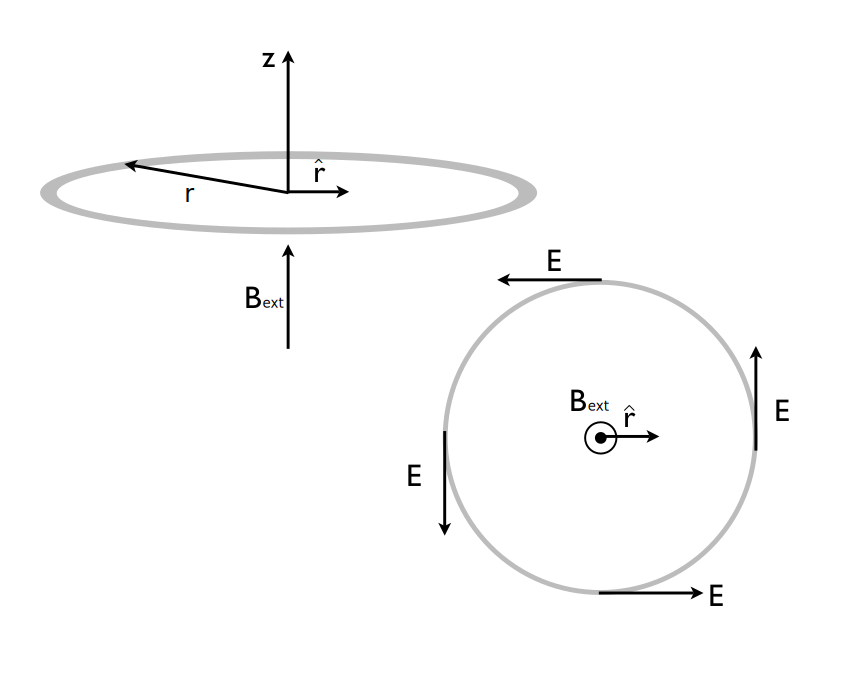
\includegraphics[width=0.4\textwidth]{corrente_tangencial.png}
	\fonte{LECLAIR, 2008}
\end{figure}

Como dito na Introdução, o anel tem um total de carga $q$ uniformemente distribuído em seu comprimento $2\pi r$, então a densidade linear de carga é $\lambda = q/(2\pi r)$ e, portanto, um elemento infinitesimal de carga é $dq = \lambda dl$. Essa notação nos permite descrever a força elétrica $d \vec{F_e}$ que surge em resposta ao campo elétrico presente em cada elemento infinitesimal de comprimento do anel como

\begin{equation} \label{lei-de-faraday-eq}
    d \vec{F_e} = dq \vec{E} = \lambda dl \vec{E}.
\end{equation}

A fim de facilitar uma compreensão mais intuitiva dessa equação (e das seguintes), incluímos uma ilustração dos elementos infinitesimais de ângulo, comprimento, e força.

\begin{figure}[htb]\label{elementos-infinitesimais-img}
    \caption{Elementos infinitesimais}
    \centering
    \includegraphics[width=0.3\textwidth]{elementos_infinitesimais.png}
	\fonte{LECLAIR, 2008}
\end{figure}

Essa figura ajuda a perceber que o campo elétrico tangente ao anel segue a igualdade $\vec{E} = E \hat{\theta}$, onde $\hat{\theta}$ é o versor no sentido em que o ângulo interno ao anel aumenta, logo

\begin{equation}
    d \vec{F_e} =  \lambda dl E \hat{\theta}.
\end{equation}

A partir disso, calculamos o torque em cada elemento de comprimento do anel. Como o fulcro está no centro no anel, o braço do torque equivale ao raio $\vec{r}$ do anel, então o elemento de torque é

\begin{equation}
    d \vec{\tau} = \vec{r} \times d\vec{F}
\end{equation}

\begin{equation}
    \Rightarrow d \vec{\tau} = \left(r \hat{r}\right) \times \left(\lambda dl E \hat{\theta}\right)
\end{equation}

\begin{equation} \label{elemento-de-torque-eq}
    \Rightarrow d \vec{\tau} = \lambda r dl E \left(\hat{r} \times \hat{\theta}\right).
\end{equation}

Pela ``Regra da Mão Direita'', o produto vetorial da equação \ref{elemento-de-torque-eq} equivale a $\hat{z}$ (isso é mais fácil de perceber se você der um ``tapa'' com a mão direita, do versor $\hat{r}$ para um dos vetores $\vec{E}$ na figura \ref{campo-tangencial-img}), então o elemento de torque é

\begin{equation}
    \Rightarrow d \vec{\tau} = \lambda r dl E \hat{z},
\end{equation}

\noindent e, portanto, o torque no anel inteiro é

\begin{equation}
    \vec{\tau} = \oint_{\text{anel}} d \vec{\tau} = \lambda r \left(\oint_{\text{anel}} dl E\right) \hat{z}.
\end{equation}

Como o campo elétrico é tangencial, $d\vec{l} \parallel \vec{E}$ em todo o anel. Por esse motivo temos $dl E = d\vec{l} \cdot \vec{E} $, então

\begin{equation}
    \vec{\tau} = \lambda r \left(\oint_{\text{anel}} d\vec{l} \cdot \vec{E}\right) \hat{z},
\end{equation}

\noindent que pela Lei de Faraday (vide equação \ref{lei-de-faraday-eq}) é

\begin{equation}
    \vec{\tau} = \left(\lambda r \Delta V \right) \hat{z}
\end{equation}

\noindent\textcolor{blue}{Dúvida: o resultado dessa integral não deveria ser $-\Delta V$? A Lei de Faraday (como expressa na equação \ref{lei-de-faraday-eq}) nos leva a esse resultado, mas a fonte que usamos para compor nossa resolução \cite{leclair_2008} indicou $\Delta V$ como resultado da integral. Isso está relacionado a direção do campo elétrico?}

\begin{equation}
    \Rightarrow \vec{\tau} = \left(\frac{q}{2\pi \cancel{r}}~\cancel{r} \Delta V \right) \hat{z} = \left(\frac{q \Delta V}{2\pi}\right) \hat{z}
\end{equation}

Agora que ajeitamos todas as direções, podemos substituir a notação vetorial pela notação escalar obtendo a equação

\begin{equation}
    \tau =  \left(\frac{q \Delta V}{2\pi}\right),
\end{equation}

\noindent que, pela Lei de Faraday, equivale a

\begin{equation}
    \tau =  - \left(\frac{q}{2\pi}\right)\frac{d \Phi_B}{d t}.
\end{equation}

Note que $q \ne 0$ e $\Delta V \ne 0$, então o torque é não-nulo e, portanto, o anel gira.

\subsection{Velocidade angular do anel}
Pela Segunda Lei de Newton, o torque resultante equivale a derivada temporal do momento angular $L$, então

\begin{equation}
    \tau = \frac{dL}{dt} =  - \left(\frac{q}{2\pi}\right)\frac{d\Phi_B}{dt}
\end{equation}

\begin{equation} \label{integral-momento-angular-eq}
    \Rightarrow \int_i^f dL = \int_i^f - \left(\frac{q}{2\pi}\right) d\Phi_B,
\end{equation}

\noindent onde os limites de integração $i$ e $f$ representam os instantes imediatamente anterior e posterior ao desligamento da corrente do solenoide, respectivamente. Resolvendo as integrais da equação \ref{integral-momento-angular-eq}, obtemos

\begin{equation}
    L_f - L_i = \frac{q}{2\pi}(\Phi_{Bi} - \Phi_{Bf}),
\end{equation}

\noindent onde $L_i = 0$ pois o momento angular inicial é nulo, e $\Phi_{Bf} = 0$ pois o campo magnético é nulo logo após o desligamento da corrente no solenoide. Assim o momento angular final do anel é

\begin{equation}
    L_f = \frac{q}{2\pi}\Phi_{Bi}
\end{equation}

\begin{equation}
    \Rightarrow L_f = \frac{q}{2\cancel{\pi}}(B_{\text{ext}}\cancel{\pi} r^2)
\end{equation}

\begin{equation}
    \Rightarrow L_f = \frac{q}{2}(B_{\text{ext}}~r^2).
\end{equation}

Sabendo que o momento de inércia $I$ de um anel de raio $r$ e massa $m$ é dado por $I = mr^2$, podemos calcular a velocidade angular $\omega$ como

\begin{equation}
    \omega = Lf/I = \frac{q}{2}\left(\frac{B_{\text{ext}}~\cancel{r^2}}{m\cancel{r^2}}\right)
\end{equation}

\begin{equation}
    \Rightarrow \omega = \frac{qB_{\text{ext}}}{2m}
\end{equation}

\subsection{Campo magnético inicial}

O momento angular de um único elétron no solenoide é

\begin{equation}
    L_{\text{elétron}} = m_e v_e b,
\end{equation}

\noindent onde $m_e$ e $v_e$ são, respectivamente, a massa e a velocidade de um elétron. Assim, o momento angular dos elétrons em uma espira do solenoide é

\begin{equation}
    L_{\text{espira}} = (n_e 2\pi b)(m_e V_e b) = n_e  2\pi b^2 m_e v_e,
\end{equation}

sendo $n_e$ o número de elétrons em uma espira. Por fim, o momento angular do total de elétrons no solenoide é

\begin{equation}
    L_{\text{total}} = (N u_a)(2\pi b^2 m_e v_e)
\end{equation}

\begin{equation}
    \frac{L_T}{u_a} = N (2\pi b^2 m_e V_e),
\end{equation}

\noindent em que $u_a$ representa uma unidade de medida arbitrária de comprimento e $N$ representa o número de espiras no solenoide. Disso, temos as seguintes equações:

\begin{equation}
    \begin{cases}
	B_{\text{ext}} = \mu_0 n i\\
	i = n_e m_e V_e\\
	B_{\text{ext}} = \mu_0 n_e v_e q_e n
    \end{cases}
\end{equation}

\begin{equation}
    \Rightarrow \frac{L_T}{u_a} = \frac{2\pi b^2}{\mu_0 q_e} B_{\text{ext}},
\end{equation}

\noindent ou seja, podemos definir uma constante $C$ tal que

\begin{equation}
    \frac{L_T}{u_a} = C B_{\text{ext}}.
\end{equation}


\begin{equation}
    \therefore B_{\text{ext}} = \frac{L_T}{u_a C}.
\end{equation}

\section{Resultados e Conclusão}

Em primeira instância, é importante ressaltar que o primeiro argumento proposto no enunciada da questão que motivou essa pesquisa está correto e o anel vai girar! Além dessa conclusão, fomos capazes de determinar a velocidade angular do anel, bem como o campo magnético inicial do problema.

\nocite{leclair_2008}

\pagebreak
\onecolumn{
\postextual
\bibliography{references}
}

\end{document}
